\subsection{Datapath Optimization} \label{subsec:dtptopti}
According to \textcite{chen_eyeriss_2017}, the data movement can often be more energy-consuming than actual computation. Smart memory management is then required to implement \acrshort{cnn} on low power device such as \acrshort{fpga}. We discover in this section various techniques for handling the Datapath on the \acrshort{fpga}.
%
%
\subsubsection{Systolic Arrays}
%
%
Systolic arrays were implemented on the first \acrshort{fpga}-based accelerators \cite{farabet_cnp_2009, gokhale_240_2014}. A static systolic array is a static array of \acrshort{pe}, controlled by the \acrshort{cpu}. Each \acrshort{pe} is involved in a part of the computation and can communicate with adjacent \acrshort{pe}s. An illustration of its principle can be found in figure \ref{fig:sytar}. The configuration can only support convolution with a kernel size $K_*$ lower than a maximal kernel size, such that $K_* \leq K_m$ (because the number of \acrshort{pe} is static). The systolic array allows spatial data reuse+ reuse between rows and columns, high clock frequency and temporal data reuse using \acrshort{fifo} queue \cite{joos_de_ter_beerst_accelerating_2019, mittal_survey_2020}.
\begin{figure}
    \centering
    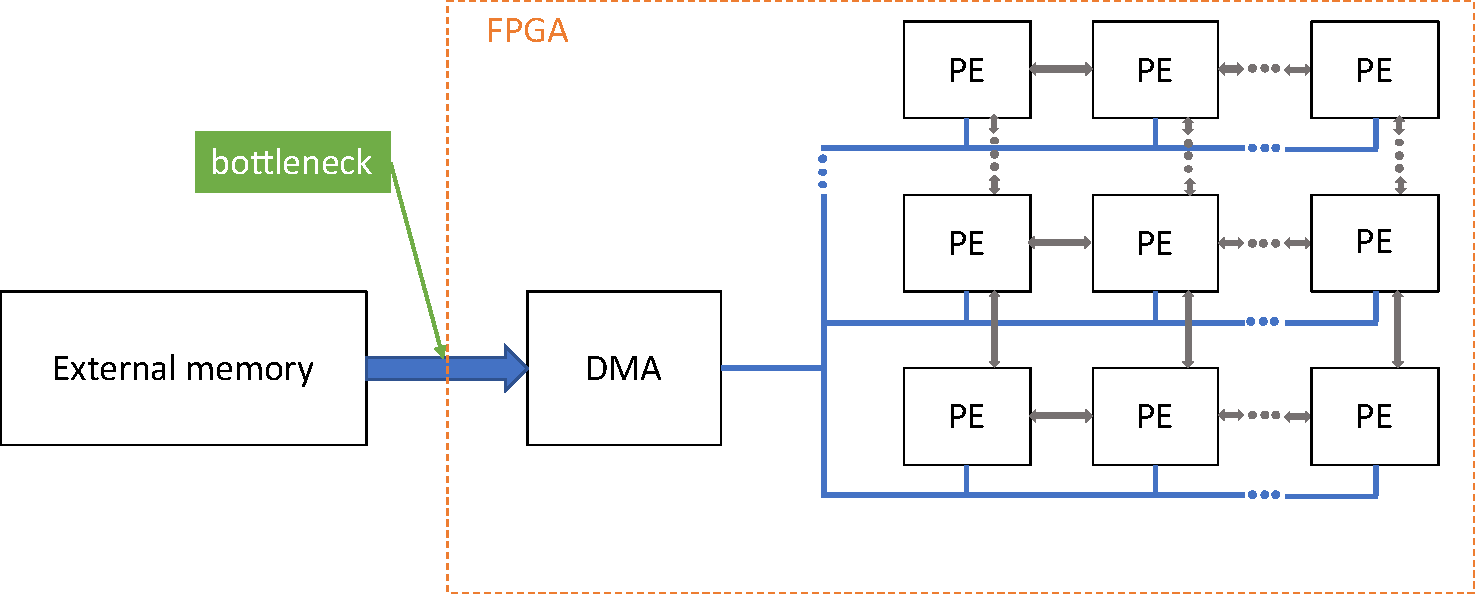
\includegraphics[width=\textwidth]{systArray.pdf}
    \caption{Static Systolic Arrays}
    \label{fig:sytar}
\end{figure} \newline \newline
However, Systolic Arrays has inefficiency problems. First, when the kernel size is much lesser than the maximal kernel size ($K_* << K_m$), there is an underutilization of the resources. For example, \cite{gokhale_240_2014} notes that for $3 \times 3$ kernels, only $9\%$ of the \acrfull{dsp} blocks are used. Second, data caching is not implemented. It means that it has always to fetch input from the external memory and it increases latency \cite{wei_automated_2017, abdelouahab_accelerating_2018}. The device performance is depending then on the memory bandwidth and it becomes memory-bounded.
%
%
\subsubsection{Data-flow MoC for CNNs (2D mapping)}
%
%
Data-flow \acrfull{moc} can be used to accelerate \acrshort{cnn}s on \acrshort{fpga}. This approach is motivated by the feed-forward aspect of the inference stage of \acrshort{cnn}, which is purely data-driven \cite{abdelouahab_accelerating_2018}. Data-flow \acrfull{moc} was firstly investigated by \cite{lin_li_low_2016}.  We can describe \acrshort{cnn} as a network where:
\begin{itemize}
    \item \textbf{nodes} are processing unit called an \textit{actor}. Each actor follows a data-driven execution where the execution is triggered by the availability of input, which is the case for a \acrshort{cnn}.
    \item \textbf{edges} are communication \acrshort{fifo} channels. Actors exchange data called \textit{tokens} through those \acrshort{fifo} channels.
\end{itemize}
A representation of a such network can be found in figure \ref{fig:moc}. \newline \newline
As the number of tokens produced and consumed by an actor can be specified in a \acrshort{cnn}, we can apply a static data-flow \cite{lee_static_1987}. The \acrshort{cnn} can be therefore modeled as a topology matrix and we only have, to minimize latency or energy consumption, to explore those matrix components (instead of tiling and unrolling parameters of section \ref{subsec:loopopti}) \cite{venieris_latency-driven_2017}. Those parameters are then used to derive \acrshort{pe} and buffer configuration. However, as pointed by \textcite{abdelouahab_tactics_2017}, is the direct hardware mapping of the \acrshort{cnn} network. It means that all the computations must be unrolled. However, we are then bounded by the hardware resources and the size of the \acrshort{cnn}, preventing implementing this approach for deep models.
\begin{figure}
    \centering
    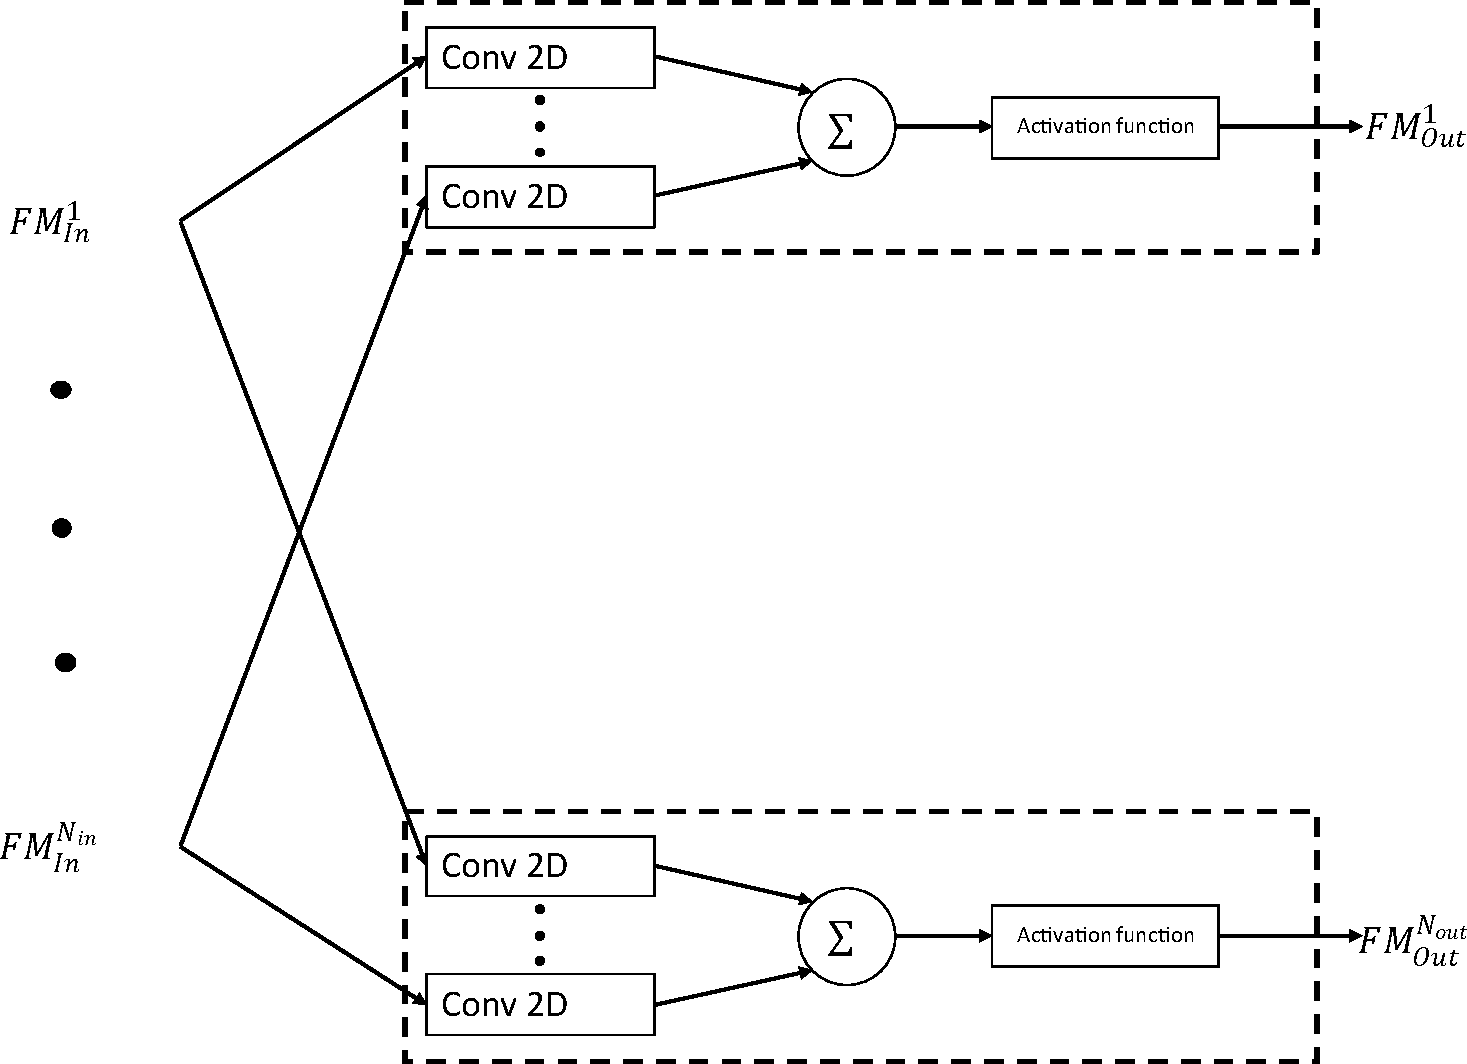
\includegraphics[width=0.8\textwidth]{Moc.pdf}
    \caption{Graph represenation of a convolution layer}
    \label{fig:moc}
\end{figure}
%
%
\subsubsection{Loop Optimization} \label{subsec:loopopti}
%
%
Loop optimizations techniques were already described in section \ref{sec:loopopti}. These techniques include parameters which can be chosen by the programmer at his will. We are going to review different works who have studied the design space exploration of unrolling parameters, tiling parameters, and loop interchange, to design the most efficient accelerator that would be feasible on the target platform. \newline \newline
%
The work of \cite{zhang_optimizing_2015} proposes an analytical solution using the roofline model \cite{williams_roofline_2009} to identify the CNN design with the best performance and lowest \acrshort{fpga} resource requirement. They have chosen a loop unrolling of ($T_{if} \times T_{of}$) to avoid complex connection topologies for all arrays. It allows spatial reuse of pixels for $T_{of}$ unrolls, and the temporal reuse of weight for ($T_{ox} \times T_{oy}$). We can observe their accelerator structure in figure \ref{lst:accelerator}. However, the disadvantage of this method is the need for a large local memory to store the partial sums ($T_{of} \times T_{ox} \times T_{oy}$).
%
\begin{figure}
    \centering
    \begin{lstlisting}[language=Java]
// Load weights
// Load input FM
% on-chip data computation
for(kx=0; kx<Nkx; kx+=1){
    for(ky=0; ky<Nky; ky+=1){
        for(tix=0; tix<min(ix+Tix, Nix); tix+=1){
            for(tiy=0; tiy<min(iy+Tiy, Niy); tiy+=1){
                for(tof=0; tof<min(of+Tof, Nof); tof+=1){
                #pragma HLS UNROLL
                    for(tif=0; tif<min(if+Tif, Nif); tif+=1){
                    #pragma HLS UNROLL
                    L : output_fm[tof][tix][tiy] +=
                    weights[tof][tif][kx][ky]*
                    input_fm[tif][S*tix+kx][S*tiy+ky];
                    }
                }
            }
        }
    }
}
// Load input FM
    \end{lstlisting}
    \caption{Architecture loop ordering \cite{zhang_optimizing_2015}}
    \label{lst:accelerator}
\end{figure} \newline
%
Once the loop ordering and unrolling parameters have been set, the roofline model can be used to find the optimal tiling parameters. \textcite{mittal_survey_2020} defines this design space exploration method as: "\textit{The roofline model relates performance to computational performance and off-chip memory traffic}". As an implementation can either be computation-bounded or memory-bounded, it uses those two limits to find the best trade-off between memory bandwidth and computational speed.
\begin{enumerate}
    \item \textbf{Computational roof}: $= \frac{\text{\# \ of \ operations}}{\# \ of \ execution \ cycles}$.
    \item \textbf{CTC ratio}: $= \frac{\text{\# \ of \ operations}}{\# \ of \ external \ data \ access}$
\end{enumerate}
Therefore, we can compute the attainable performance as equation \ref{eq:atperf}.
\begin{equation}
Att \ perf = min \ (Computational \ roof; CTC \ ratio \times bandwidth)
\label{eq:atperf}
\end{equation}
The roofline method is shown in figure \ref{fig:roofmeth}. In this figure, implementations C and D achieves the highest possible performance on the \acrshort{fpga}. However, implementation C is preferred because it requires the least bandwidth.
%
\begin{figure}
    \centering
    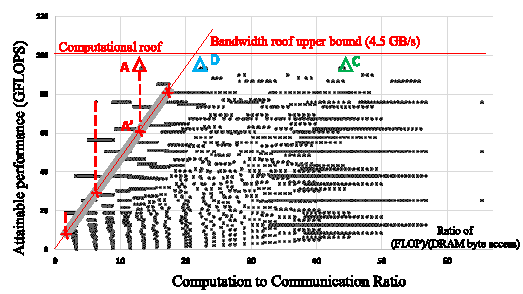
\includegraphics[width=\textwidth]{roofmethod.pdf}
    \caption{Design space of platform-supported designs  \cite{zhang_optimizing_2015}}
    \label{fig:roofmeth}
\end{figure} \newline \newline
%
\cite{motamedi_placid_2017} chooses the best parameters according to its resources and the data reuse scheme. They do not tile on the kernel and on the spatial axis because the on-chip memory is larger than an \acrshort{fm} size and recent \acrshort{cnn} have small filters, and to avoid the problem of loading multiple times the same pixel. As the tile goes over the input and output \acrshort{fm} channel, we can choose between maximizing the reuse of the input \acrshort{fm} (MIR, each \acrshort{fm} is loaded once but some intermediate results have to be wrote back to memory) or output \acrshort{fm} (MOR, we avoid writing back intermediate results to memory but some input \acrshort{fm} have to be loaded more than once). Then they perform an exhaustive search on the tiling and \acrshort{pe} parameters to find the optimal design. It can be layer-specific (but the \acrshort{fpga} needs dynamic reconfiguration and \textcite{zhang_optimizing_2015} have proven it is inefficient) or values are fixed for all layer.
%
A different approach has been studied by \cite{ma_optimizing_2018}. It proposes a design space exploration regarding the various design objectives. They have proposed two flowcharts in figure \ref{fig:flowchart} to
\begin{itemize}
    \item \textbf{Latency}: $P_*$ should be common factors of  $T_*$ for all convolution layers to fully utilize \acrshort{pe}s, and $T_*$ to be the common factors of  $N_*$ to make full use of external memory transactions.
    \item \textbf{Partial sum storage}: to minimize the concurrent storage of partial sums in local memory and allowing to keep them into the PE, we should prior the computation of an output pixel to evacuate it to the external memory.
    \item \textbf{On-chip memory access}: on-chip memory access can be minimized by reusing at most pixels or weights in the \acrshort{pe}s.
    \item \textbf{External memory access}: to minimize external access, a sufficient buffer size should be assigned to pixels and weights.
\end{itemize}
%
\begin{figure}
\centering
    \begin{subfigure}{.45\textwidth}
    \centering
    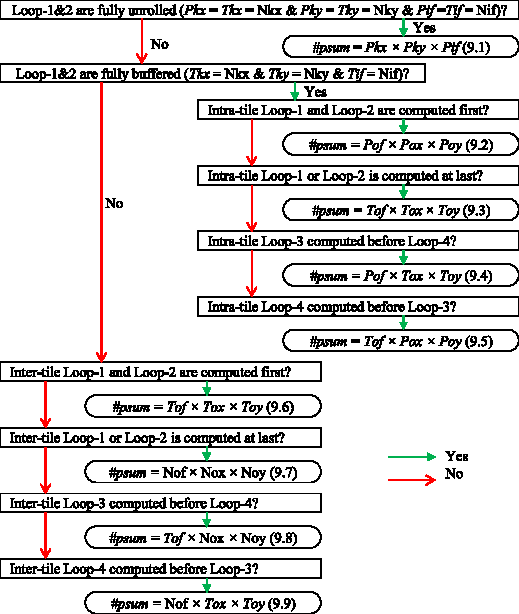
\includegraphics[width=\linewidth]{fwch1.pdf}
    \caption{ }
    \end{subfigure}
    \begin{subfigure}{.45\textwidth}
    \centering
    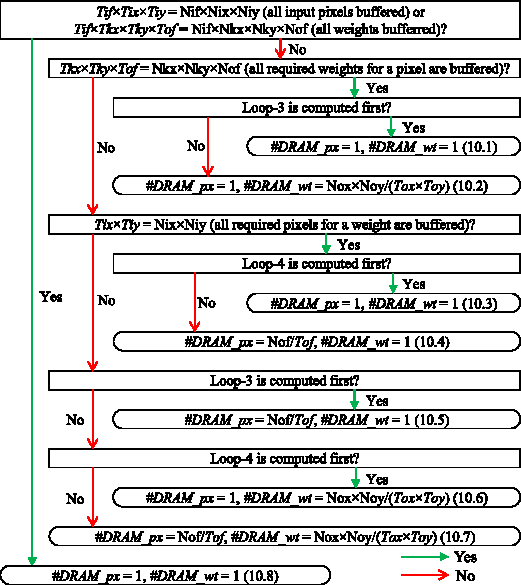
\includegraphics[width=\linewidth]{fwch2.pdf}
    \caption{ }
    \end{subfigure}
    \caption{Design space exploration of: (a) total number of partial sums that need to be stored in memory; (b) the number of external memory accesses \cite{ma_optimizing_2018}}
    \label{fig:flowchart}
\end{figure}
